\section{Simulation Results}

% \setlength{\abovedisplayskip}{-5pt} \setlength{\abovedisplayshortskip}{-5pt}
\setlength{\belowdisplayskip}{5pt} \setlength{\belowdisplayshortskip}{5pt}

\setlength{\textfloatsep }{-2.5pt}
\setlength{\floatsep }{-2.5pt}

\setlength{\dbltextfloatsep }{-0pt}
\setlength{\dblfloatsep }{-5pt}

In this section, we incorporate the linearized three phase power flow model into an OPF program.  The goal of the optimization is to control inverter VAR resources in a distribution system to regulate and balance system voltages.  We define the problem as:

\begin{equation}
\begin{aligned}
& \underset{u,y_{i},Q_{i},P_{i}}{\text{minimize}}
% & & P_{0}\\
& & \sum_{i \in H} \left[ \sum_{ \substack{ {\phi, \psi \in \{ a,b,c\}} \\ {\phi \neq \psi} }} ( y_{\phi,i} - y_{\psi,i} )^{2}\right] + \rho u_{\phi,i}^2   \\
& \text{subject to}
& & ~\eqref{eq:mag_8}-\eqref{eq:pow_4}, \\
& & & \underline{y} \le y_{i} \le \overline{y}, \quad  \forall i \in H, 
\end{aligned} \label{eq:opt}
\end{equation}

\noindent where $\rho$ is positive ($0.5$ in simulations) and $\underline{y}$ and $\overline{y}$ represent upper and lower bounds on voltage magnitude (which are fixed to $0.95^{2}$ and $1.05^{2}$), respectively. The first term in the objective function is the sum squared Euclidean distances of squared voltage magnitude differences across phases at each node. The second term penalizes the use of inverter VAR resources.

The OPF is performed on the IEEE 13 test node distribution feeder \cite{IEEEtestfeeder}, seen in Fig. \ref{fig:13node}.  This simulation neglects the presence of the voltage regulator between nodes 650 and 632, the transformer between nodes 633 and 634, the switch (assumed closed) between nodes 671 and 692, and capacitors at nodes 675 and 611. Constant power and constant impedance load fractions were assigned as $a_{i}^{0} = 0.85$ and $a_{i}^{1} = 0.15$.

\begin{figure}[t]
\centering
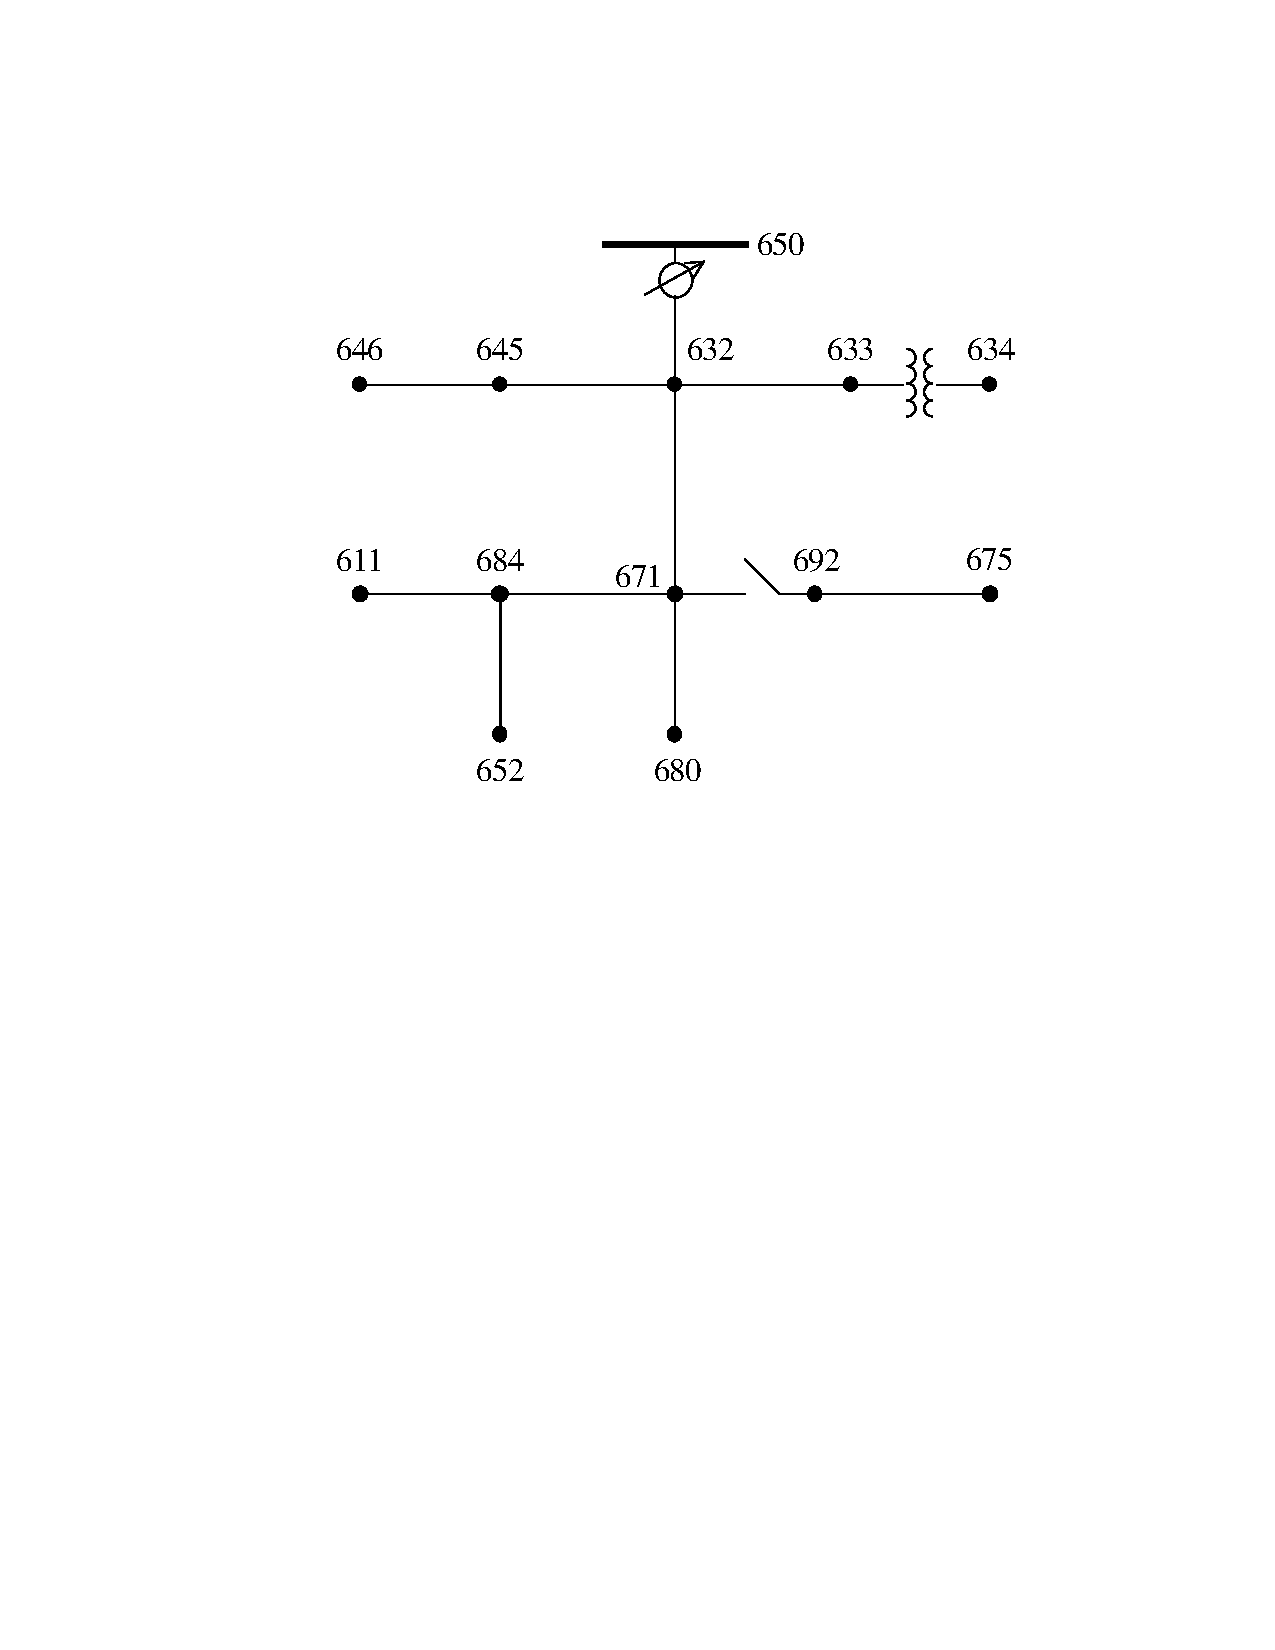
\includegraphics[width=3.0in]{13_node_feeder.pdf}
\caption{IEEE 13 node feeder model.}
\label{fig:13node}
\end{figure}

Feeder configurations, per-length line segment impedances, and line segment lengths can be found in \cite{IEEEtestfeeder}.  All line segment impedances were increased by a factor of 1.25. Spot loads (also found in \cite{IEEEtestfeeder}) were assigned to nodes according to Table \ref{tab:loads}. Distributed loads were neglected.  For the simulation, feeder power and voltage base values were chosen as the power rating and secondary voltage of the substation transformer, 500kVA and 4.16kV respectively.  Additionally, feeder head voltage was fixed to 1 p.u..  Controllable three phase inverter resources were placed at nodes 632, 675, 680, and 684.  These resources were purposefully left unconstrained to test the effectiveness of the OPF, with the ability to source or sink arbitrary amounts of reactive power. 

\begin{table}[h]
	\caption{SPOT LOADS OF 13 NODE FEEDER.}	
	\begin{center}
		\begin{tabular}{| l | c | c | c |}
        	\hline
        	& \multicolumn{3}{|c|}{Phase } \\
        	\hline
        	Node & $a$ [pu] & $b$ [pu] & $c$ [pu] \\
            \hline
			650 & 0 & 0 & 0 \\
            \hline
            632 & 0 & 0 & 0 \\
            \hline
            633 & 0 & 0 & 0 \\
            \hline
            634 & 0.032 + j 0.022 & 0.024 + j 0.018 & 0.024 + j 0.018 \\
            \hline
            645 & -- & 0.034 + j 0.025 & 0 \\
            \hline
            646 & -- & 0.046 + j 0.0264 & 0 \\
            \hline
            671 & 0.077 + j 0.044 & 0.077 + j 0.044 & 0.077 + j 0.044 \\
            \hline
            692 & 0 & 0 & 0.034 + j 0.0302 \\
            \hline
            675 & 0.097 + j 0.038 & 0.0136 + j 0.012 & 0.058 + j 0.0424 \\
            \hline
            680 & 0 & 0 & 0 \\
            \hline
            684 & 0 & -- & 0 \\
            \hline
            652 & 0.0256 + j 0.0172 & -- & -- \\
            \hline
            611 & -- & -- & 0.034 + j 0.0106 \\
            \hline
            Total & 0.2316 + j 0.1212 & 0.1946 + j 0.1254 & 0.227 + j 0.1506 \\
            \hline
		\end{tabular}
	\end{center}	
	\label{tab:loads}
\end{table}

Simulation results are presented in Figs. \ref{fig:Vres} - \ref{fig:unode} and in Table \ref{tab:unode}.  Voltage profiles for the base scenario (where inverter VAR resources are not utilized) and control scenario (inverter VAR resources are determined by the OPF of \eqref{eq:opt}) can be seen in Fig. \ref{fig:Vres}, with phase $a$, $b$ and $c$ voltage magnitudes plotted in Fig. \ref{fig:Va}, Fig. \ref{fig:Vb}, and Fig. \ref{fig:Vc}, respectively. As the figures show, in the control case, the voltage magnitudes of phase $a$ are kept almost constant with the base case. The voltage magnitudes of phase $b$ are decreased, and of $c$ are increased, to achieve greater voltage magnitude balance. Additionally, the voltages of phase $c$, originally in violation of the lower voltage bound, are now within the acceptable $\pm 5\%$ threshold.  It should be noted that the rise in voltage magnitude for the base scenario from node 632 to node 671 reconciles with power-flow simulation results in \cite{IEEEtestfeeder} and is likely due to the fact that off diagonal components of \eqref{eq:M}-\eqref{eq:N} have \emph{opposite} signs of the diagonal components, indicating that large voltage drops in some phases actually contribute to voltage \emph{rises} in other phases.

% As the figures show, in the control case the voltage magnitudes of phases $a$ and $c$ are increased compared to the base case, whereas the magnitudes of phase $b$ are decreased.  Additionally, the voltages of phase $c$, originally in violation of the lower voltage bound, are now within the acceptable $\pm 5\%$ threshold.

A comparison of voltage magnitudes for all phases at each node can be seen in Fig. \ref{fig:VbaseVcon}, with the base scenario in Fig. \ref{fig:Vbase}, and the control scenario in Fig. \ref{fig:Vcon}.  As the figures show, the voltage magnitudes are much closer together when inverter reactive power is dispatched according to the results of the OPF of \eqref{eq:opt}.

Figure \ref{fig:Vbalance} evaluates the first term of objective function of \eqref{eq:opt} for all nodes with and without control action.  The results show that the objective function value (which measures the Euclidian distance between squared voltage magnitudes) decreases at all nodes following control action with the exception of node 646, which increases very slightly.  

Optimal inverter control output is shown in Fig. \ref{fig:unode} and listed in \ref{tab:unode}.  As the figure shows, to balance the system, inverters at node 675 and 632 actually \emph{consume} VARs.  We believe that this effect occurs as these phase voltages are increasing compared to voltages in the remaining phases.

\begin{table}[h]
	\caption{OPTIMAL INVERTER VAR DISPATCH.}	
	\begin{center}
		\begin{tabular}{| l | c | c | c |}
        	\hline
        	& \multicolumn{3}{|c|}{Phase } \\
        	\hline
        	Node & $a$ [pu] & $b$ [pu] & $c$ [pu] \\
            \hline
% 			650 & 0 & 0 & 0 \\
%             \hline
            632 & -0.0081 & -0.0346 & 0.0437 \\
            \hline
%             633 & 0 & 0 & 0 \\
%             \hline
%             634 & 0 & 0 + j 0 \\
%             \hline
%             645 & 0 & 0 & 0 \\
%             \hline
%             646 & 0 & 0 & 0 \\
%             \hline
%             671 & 0 & 0 & 0 \\
%             \hline
%             692 & 0 & 0 & 0 \\
%             \hline
            675 & 0.005 & 0.0522 & -0.058 \\
            \hline
            680 & 0.003 & 0.0011 & -0.0038 \\
            \hline
            684 & -0.0003 & -- & -0.0389 \\
            \hline
%             652 & 0 & 0 & 0 \\
%             \hline
%             611 & 0 & 0 & 0 \\
%             \hline
            Total & -0.0003 & 0.0187 & -0.057 \\
            \hline
		\end{tabular}
	\end{center}	
	\label{tab:unode}
\end{table}

% We define a metric of voltage magnitude imbalance at a node as the Euclidean norm of all possible voltage magnitude differences at the node, as in \eqref{eq:imbal}. The imbalance for the base and control scenarios are shown in Fig. \ref{fig:Vbalance}.

% The total imbalance of the feeder is given by $\sum_{k \in H} J_{k}$, with a base scenario value of 0.3352 and control scenario value of 0.0283.

% \begin{equation}
% 	J_{k} = \left[ \sum_{ \substack{ {\phi, \psi \in \Phi_{i}} \\ {\phi \neq \psi} }} \left( \left| V_{\phi,k} \right| - \left| V_{\psi,k} \right| \right)^2 \right]^{1/2}
%     \label{eq:imbal}
% \end{equation}

% \begin{table}[!htb]
% 	\caption{COMPARISON OF FEEDER HEAD POWER FOR BASE AND CONTROL SCENARIOS.}	
% 	\begin{center}
% 		\begin{tabular}{| l c | c | c |}
%         	\hline
%         	& & Base scenario [pu] & Control Scenario [pu] \\
%             \hline
% 			Apparent Power & $S_{0}$ & 0.7842 & 0.7648 \\
%             \hline
%             Real Power & $P_{0}$ & 0.6588 & 0.6584 \\
%             \hline
%             Reactive Power & $Q_{0}$ & 0.4243 & 0.3824 \\
%             \hline
% 		\end{tabular}
% 	\end{center}	
% 	\label{tab:pow}
% \end{table}

% \begin{table}[!htb]
% 	\caption{DER CONTROL INPUTS.}	
% 	\begin{center}
% 		\begin{tabular}{| l | c | c | c |}
%         	\hline
%         	& \multicolumn{3}{|c|}{Phase } \\
%         	\hline
%         	Node & $a$ [VAr pu] & $b$ [VAr pu] & $c$ [VAr pu] \\
%             \hline
% 			632 & & & \\
%             \hline
%             675 & & &  \\
%             \hline
%             680 & & &  \\
%             \hline
%             684 & & & \\
%             \hline
% 		\end{tabular}
% 	\end{center}	
% 	\label{tab:uk}
% \end{table}

\begin{figure}[t]
\centering
\begin{subfigure}[b]{0.49\textwidth}
	\centering
	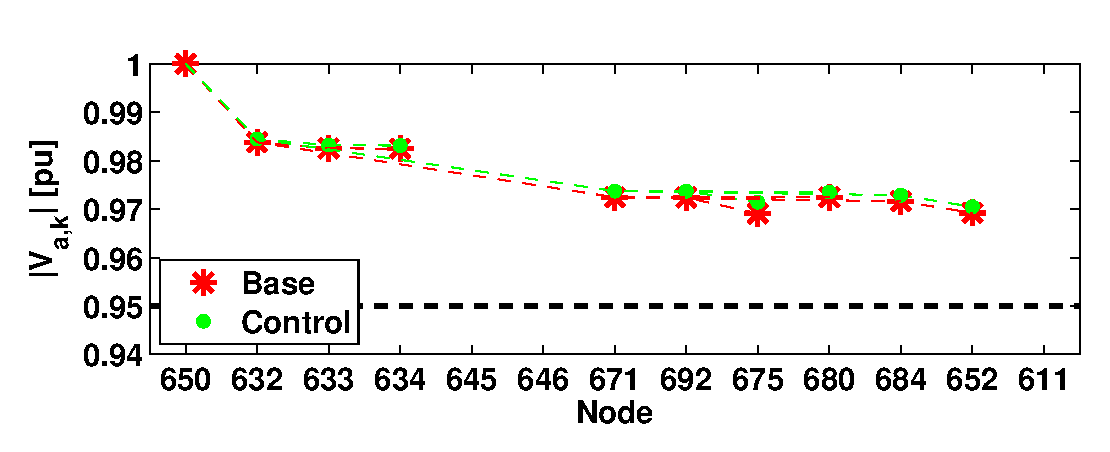
\includegraphics[width=\textwidth]{Va.eps}
	\caption{Phase $a$ voltage magnitudes.}
	\label{fig:Va}
\end{subfigure}
\\
\begin{subfigure}[b]{0.49\textwidth}
	\centering
	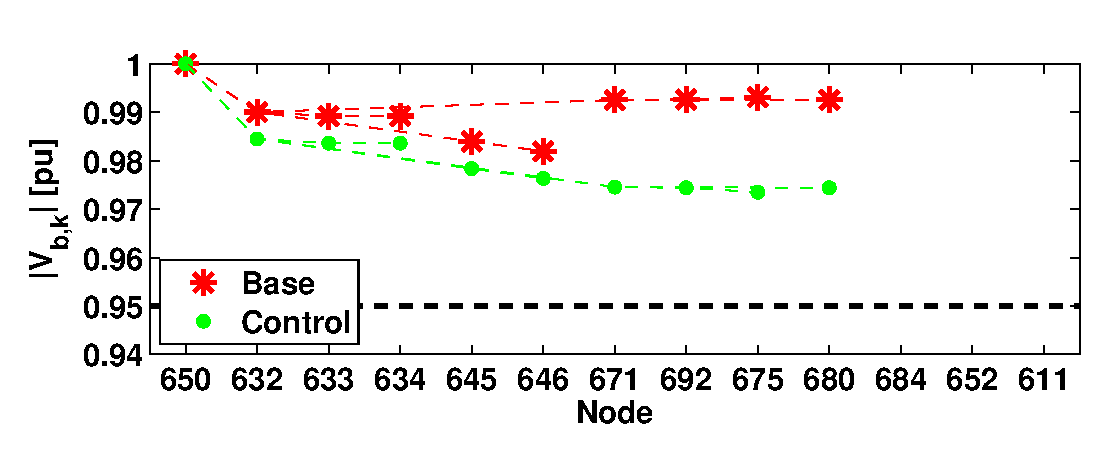
\includegraphics[width=\textwidth]{Vb.eps}
	\caption{Phase $b$ voltage magnitudes.}
	\label{fig:Vb}
\end{subfigure}
\\
\begin{subfigure}[b]{0.49\textwidth}
	\centering
	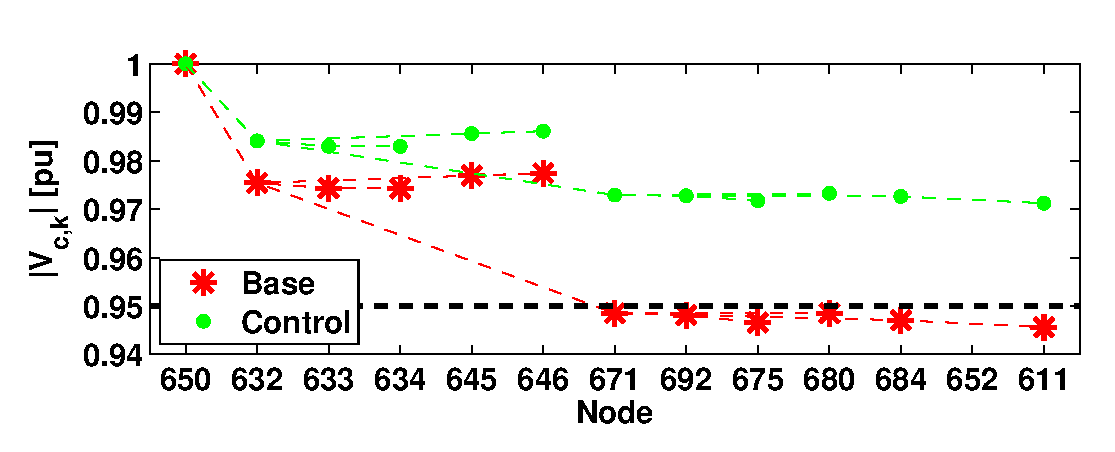
\includegraphics[width=\textwidth]{Vc.eps}
	\caption{Phase $c$ voltage magnitudes.}
	\label{fig:Vc}
\end{subfigure}
\caption{Phase $a$, $b$, and $c$ voltages magnitudes for base and control scenarios plotted individually. Dashed lines represent line segments between nodes.}
\label{fig:Vres}
\end{figure}

% \begin{figure}[t]
% 	\centering
% 	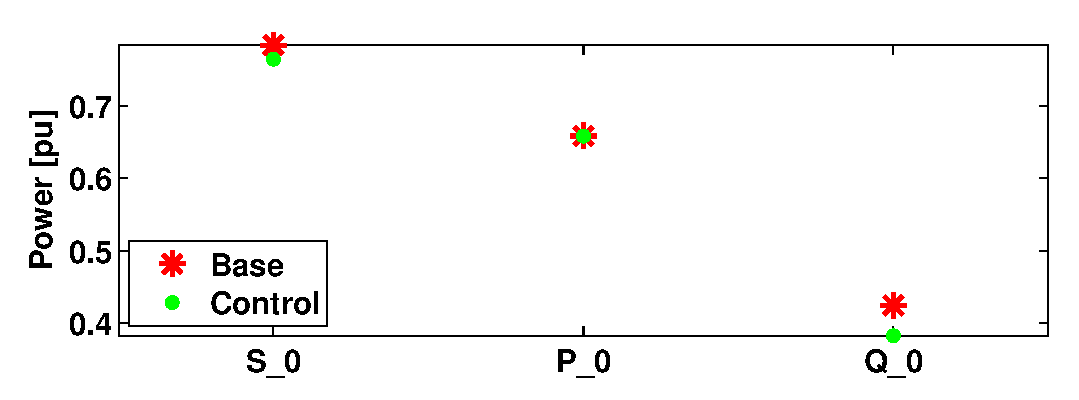
\includegraphics[width=0.5\textwidth]{SPQ.eps}
% 	\caption{Feeder head apparent, real and reactive power for the base and control scenarios.}
% 	\label{fig:SPQ}
% \end{figure}

\begin{figure*}[t]
	\centering
	\begin{subfigure}[b]{0.49\textwidth}
		\centering
		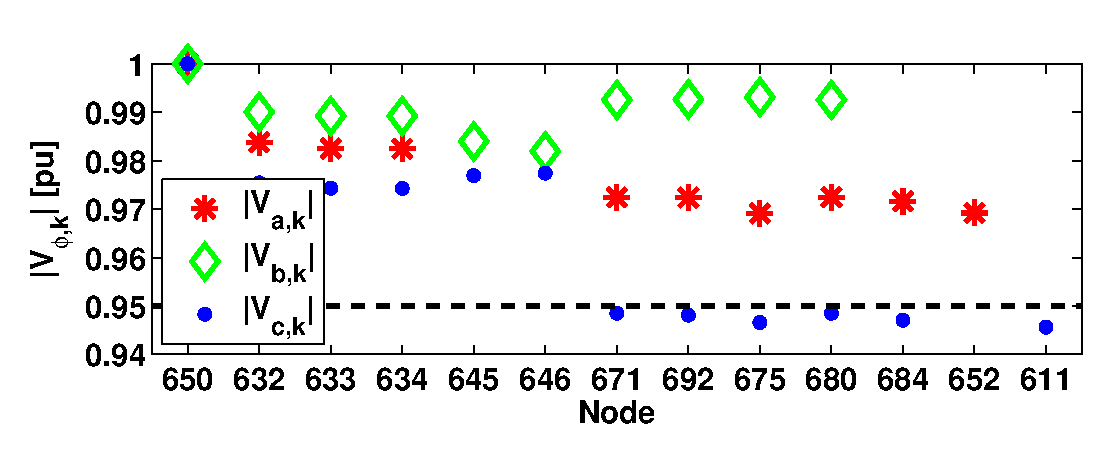
\includegraphics[width=\textwidth]{Vbase.eps}
		\caption{Voltage magnitudes without control.}
		\label{fig:Vbase}
	\end{subfigure}
    \begin{subfigure}[b]{0.49\textwidth}
		\centering
		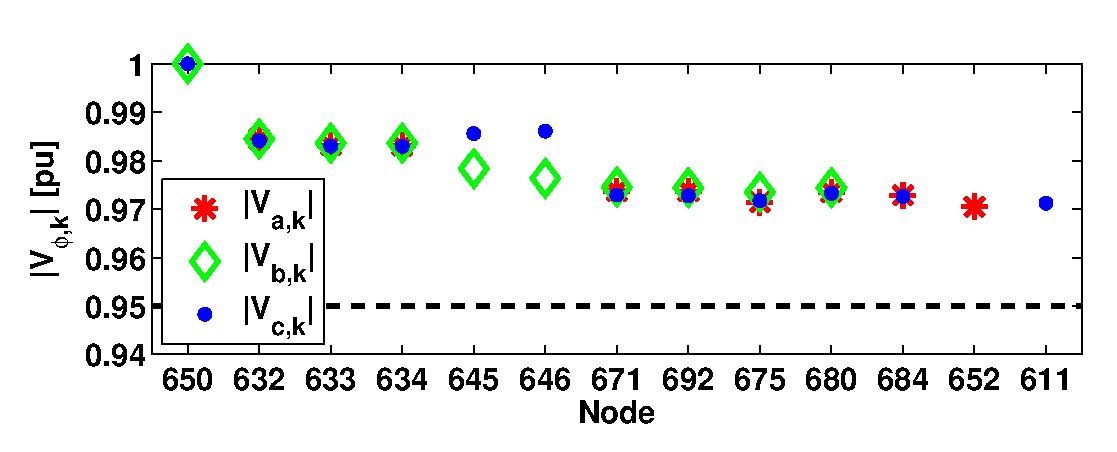
\includegraphics[width=\textwidth]{Vcon.eps}
		\caption{Voltage magnitudes with control.}
		\label{fig:Vcon}
	\end{subfigure}
    \caption{Phase $a$, $b$, and $c$ voltages magnitudes plotted together for base and control scenarios.}
	\label{fig:VbaseVcon}
\end{figure*}

\begin{figure}[t]
	\centering
	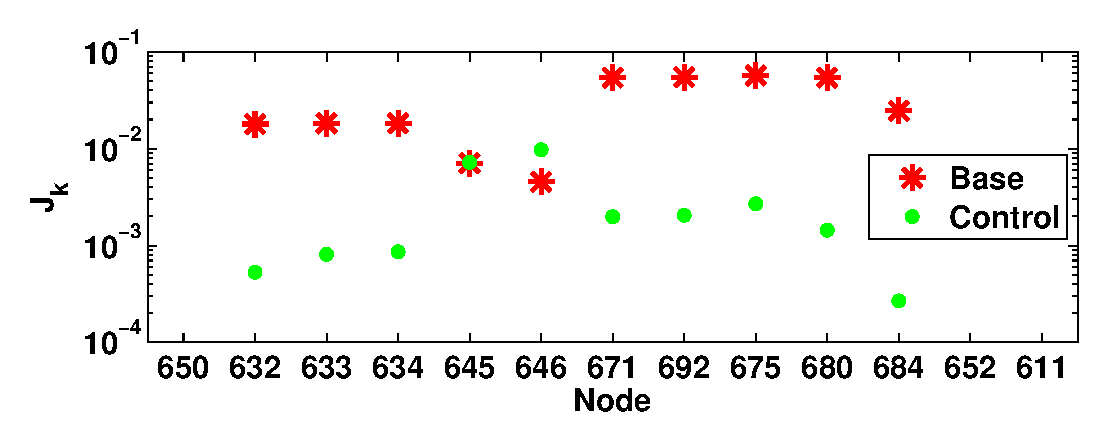
\includegraphics[width=0.5\textwidth]{Vbalance.eps}
	\caption{Phase voltage imbalance for all nodes, as defined in \eqref{eq:opt}.}
	\label{fig:Vbalance}
\end{figure}

\begin{figure}[t]
	\centering
	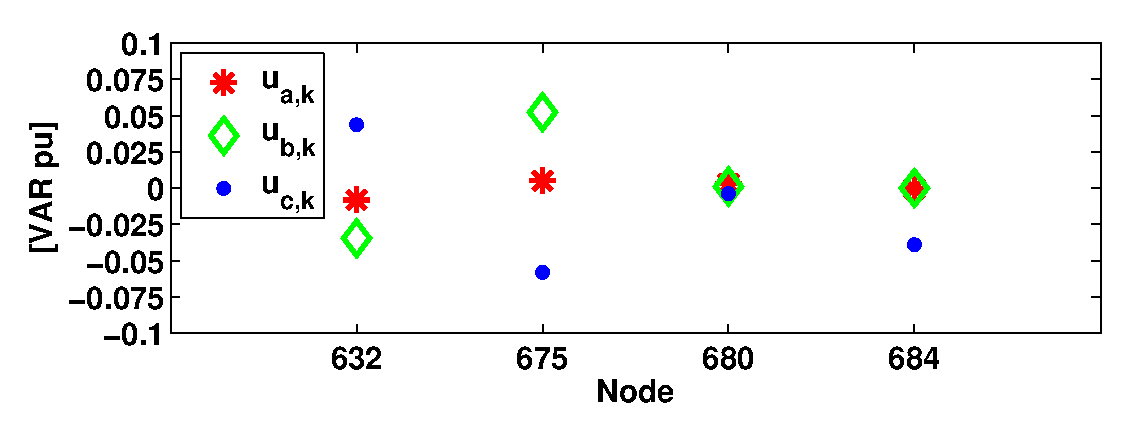
\includegraphics[width=0.5\textwidth]{unode.eps}
	\caption{Optimal inverter VAR resource.}
	\label{fig:unode}
\end{figure}